\documentclass{article}
\usepackage[T1]{fontenc}
\usepackage[utf8]{inputenc}
\usepackage{caption}
\usepackage{subcaption}
% \usepackage[htt]{hyphenat}
\usepackage{multicol}
\usepackage{float}
\usepackage{graphicx}
\usepackage{booktabs}
\usepackage{float}
\usepackage{commath}
\usepackage{pgfplots}
\usepackage{amsmath}
\usepackage{listings}
\usepackage{bm}
\usepackage{xcolor}
\usepackage[euler]{textgreek}
\usepackage{amsfonts}
\usepackage{amssymb}
\usepackage{syntax}
% \usepackage{enumitem}
% \usepackage [english]{babel}
% \usepackage [autostyle, english = american]{csquotes}
% \MakeOuterQuote{"}
% \usepackage[linguistics]{forest}
% \usetikzlibrary{trees}

\definecolor{mygreen}{RGB}{28,172,0} % color values Red, Green, Blue
\definecolor{mylilas}{RGB}{170,55,241}
%-------------------------------------------
\setlength{\textwidth}{7.0in}
\setlength{\oddsidemargin}{-0.35in}
\setlength{\topmargin}{-0.5in}
\setlength{\textheight}{9.0in}
\setlength{\parindent}{0.3in}
\title{IE 306 - Homework 2}
\author{Mehdi Saffar - 2016400411 \\ Burak Berk Ozer - 2016400015 \\ Mehmet Umut Oksuz - 2016400096}

\begin{document}
\maketitle

\section{Introduction}
In this project, we are given the observed interarrival times of customers to a
system and we are tasked to find the best-fitting random distribution. To do
that we will compare the empirical data with two of possible distributions:
uniform distribution and exponential distribution. We will use various
statistical tests to find the most fitting one.

\section{Kolmogorov-Smirnov test}
For days 1 and 2 we have applied the Kolmogorov-Smirnov test to see if it is
possible for that data to be uniformly distributed between 0 and 400. To scale
the data, first we have divided all the data with 400. And then we calculated
values for $R(i)$, $i/N$, $i/N-R(i)$ and  $R(i)-(i-1)/N$. After getting all these
values, we get the maximum and determine our KS statistic. According to our KS
statistic, using a 0.05 significance level we have concluded that data for both
days cannot come from a uniform distribution. All the details of our
Kolmogorov-Smirnov test can be found in our Excel file.
\section{Dataset statistcs}

\begin{table}[H]
    \centering
    \begin{tabular}{@{}lllllllll@{}}
        \toprule
                       & \textbf{count} & \textbf{mean} & \textbf{std} & \textbf{min} & \textbf{25\%} & \textbf{50\%} & \textbf{75\%} & \textbf{max} \\ \midrule
        \textbf{Day 1} & 488            & 44.752        & 52.804       & 1            & 13            & 26            & 54            & 434          \\
        \textbf{Day 2} & 488            & 53.801        & 55.092       & 0            & 15            & 35            & 69.25         & 339          \\ \bottomrule
    \end{tabular}
\end{table}

\section{Frequency histograms}

\begin{figure}[H]
    \begin{subfigure}{0.5\textwidth}
        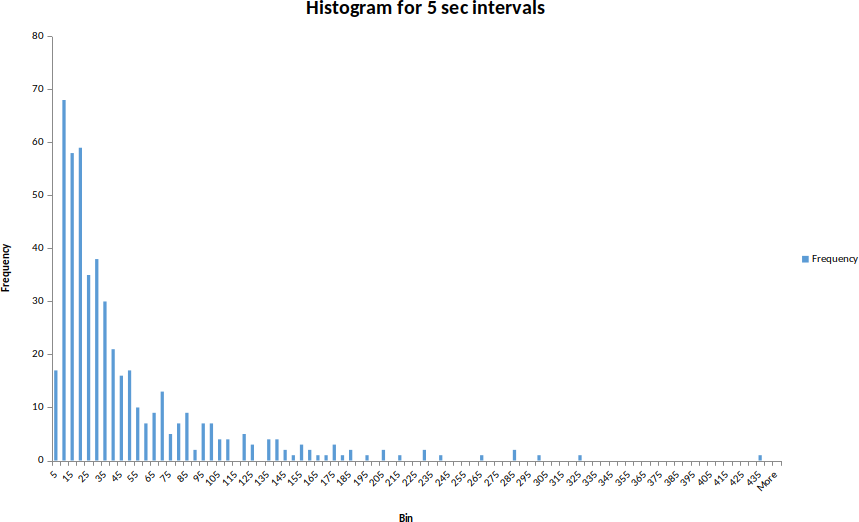
\includegraphics[width=\linewidth]{day1-hist-5sec.png}
        \caption{Frequency histogram 5 seconds intervals of day 1}
    \end{subfigure}
    \begin{subfigure} {0.5\textwidth}
        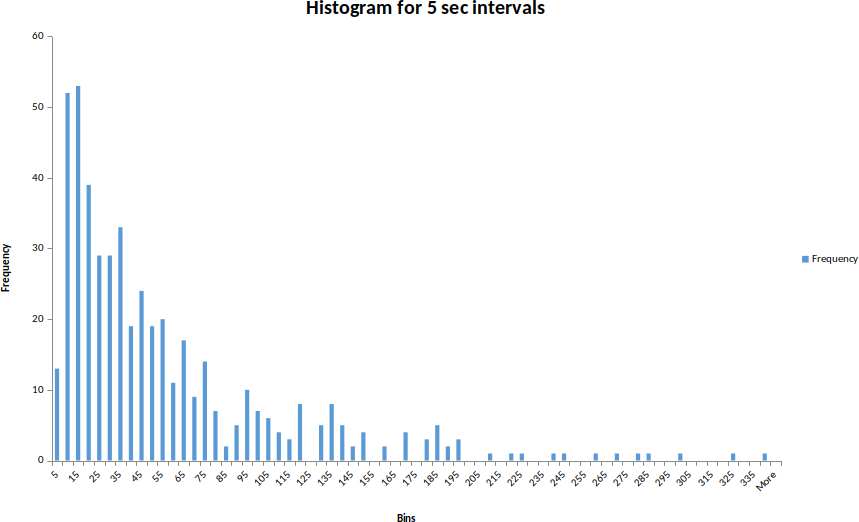
\includegraphics[width=\linewidth]{day2-hist-5sec.png}
        \caption{Frequency histogram 5 seconds intervals of day 2}
    \end{subfigure}
\end{figure}

\begin{figure}[H]
    \begin{subfigure}{0.5\textwidth}
        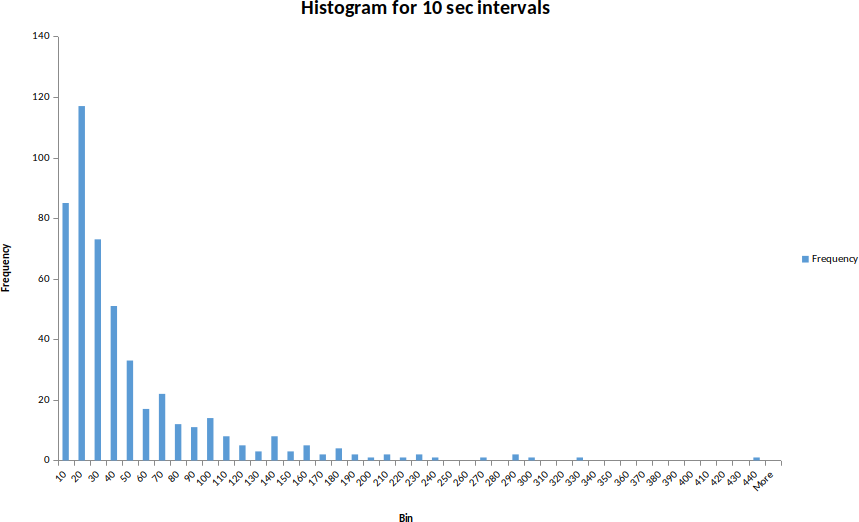
\includegraphics[width=\linewidth]{day1-hist-10sec.png}
        \caption{Frequency histogram 10 seconds intervals of day 1}
    \end{subfigure}
    \begin{subfigure} {0.5\textwidth}
        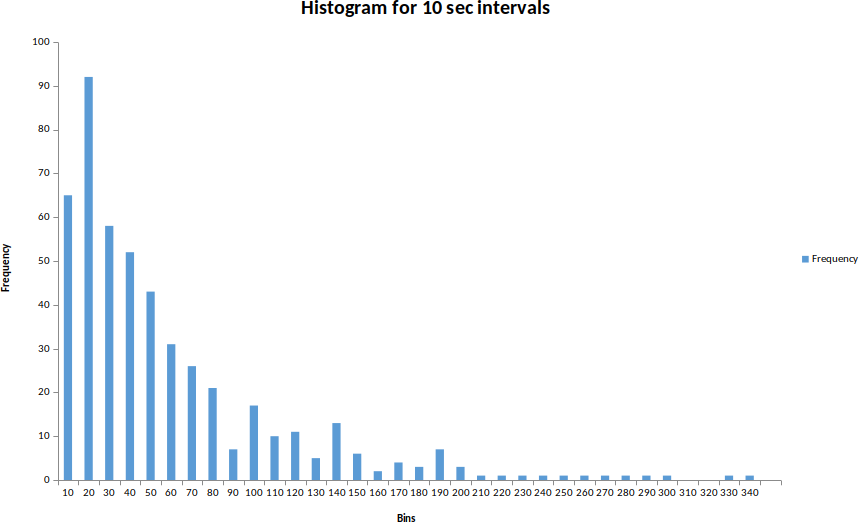
\includegraphics[width=\linewidth]{day2-hist-10sec.png}
        \caption{Frequency histogram 10 seconds intervals of day 2}
    \end{subfigure}
\end{figure}

\begin{figure}[H]
    \begin{subfigure}{0.5\textwidth}
        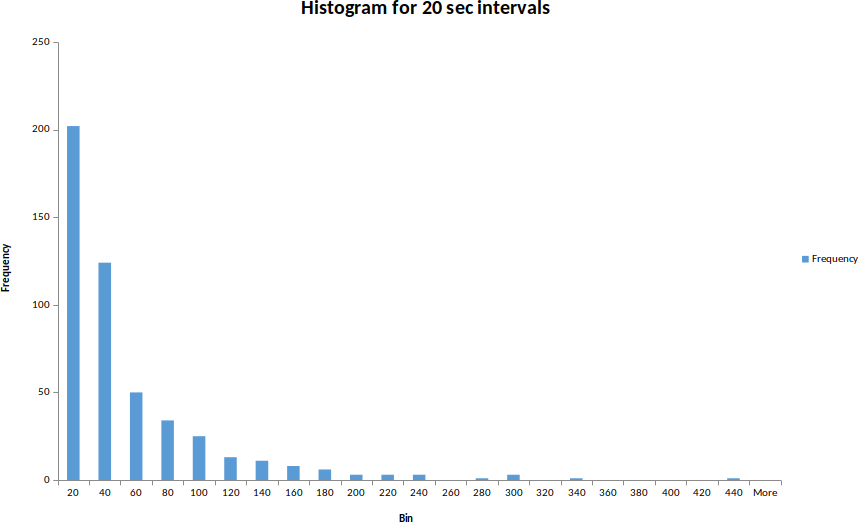
\includegraphics[width=\linewidth]{day1-hist-20sec.png}
        \caption{Frequency histogram 20 seconds intervals of day 1}
    \end{subfigure}
    \begin{subfigure}{0.5\textwidth}
        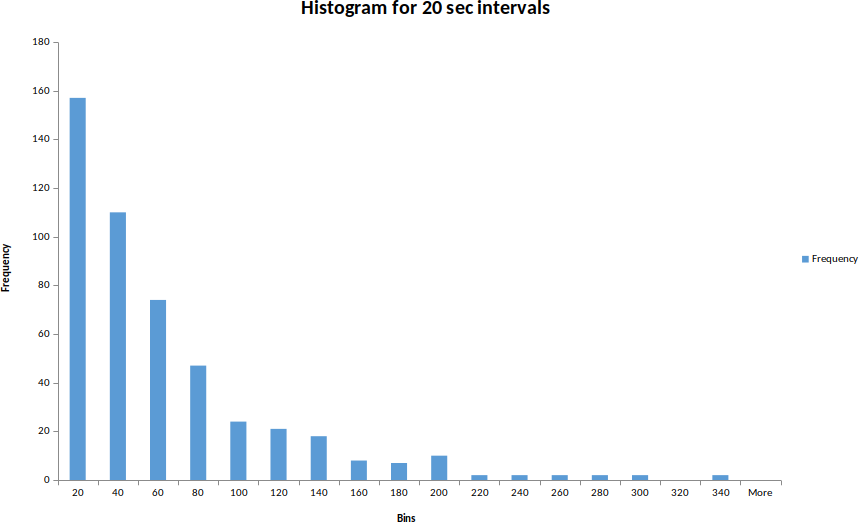
\includegraphics[width=\linewidth]{day2-hist-20sec.png}
        \caption{Frequency histogram 20 seconds intervals of day 2}
    \end{subfigure}
\end{figure}

\newpage

\section{Chi-Squared test}
We have conducted a Chi-Squared test for both days separately. We used 10 second intervals as
expected and determined our bins accordingly. Frequencies and expected frequencies of all bins
are calculated and according to those values Chi-Squared statistic is determined. For both days,
we see that our Chi-Squared statistc is smaller than the table value. So, we cannot reject the
hypothesis that this data are coming from an exponential distribution with means specified in
section 3 of the report.

\section{QQ-Plot}

\begin{figure}[H]
    \begin{subfigure}{0.5\textwidth}
        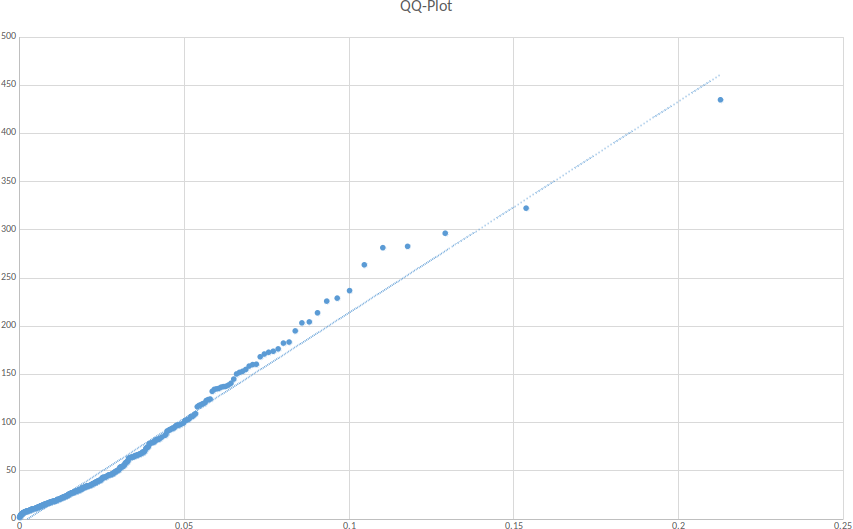
\includegraphics[width=\linewidth]{day1-qqplot.png}
        \caption{QQ-Plot of day 1}
    \end{subfigure}
    \begin{subfigure}{0.5\textwidth}
        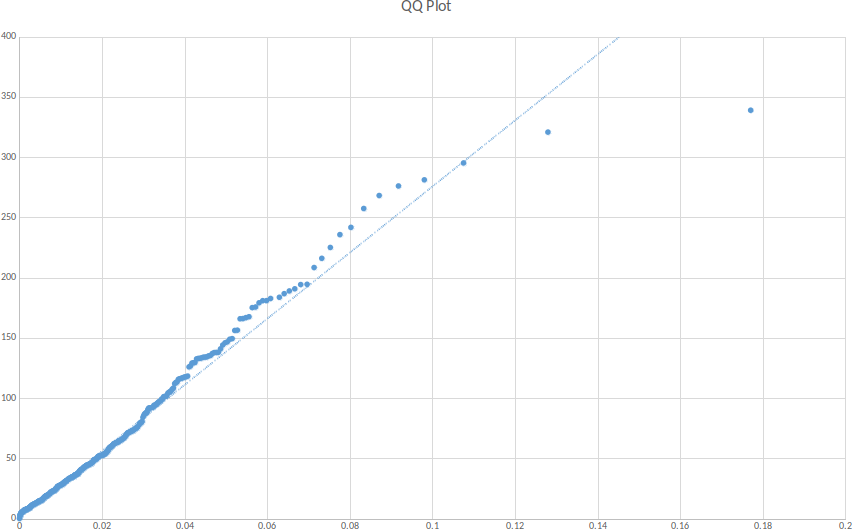
\includegraphics[width=\linewidth]{day2-qqplot.png}
        \caption{QQ-Plot of day 2}
    \end{subfigure}
\end{figure}


\section{Interarrival time plot}

\begin{figure}[H]
    \begin{subfigure}{0.5\textwidth}
        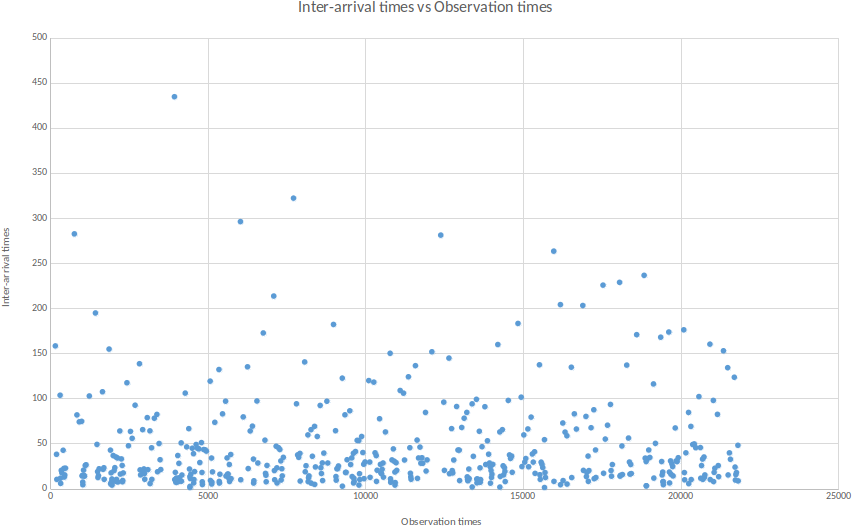
\includegraphics[width=\linewidth]{day1-interarrival-timeseries.png}
        \caption{Interarrival time vs Observer times for day 1}
    \end{subfigure}
    \begin{subfigure}{0.5\textwidth}
        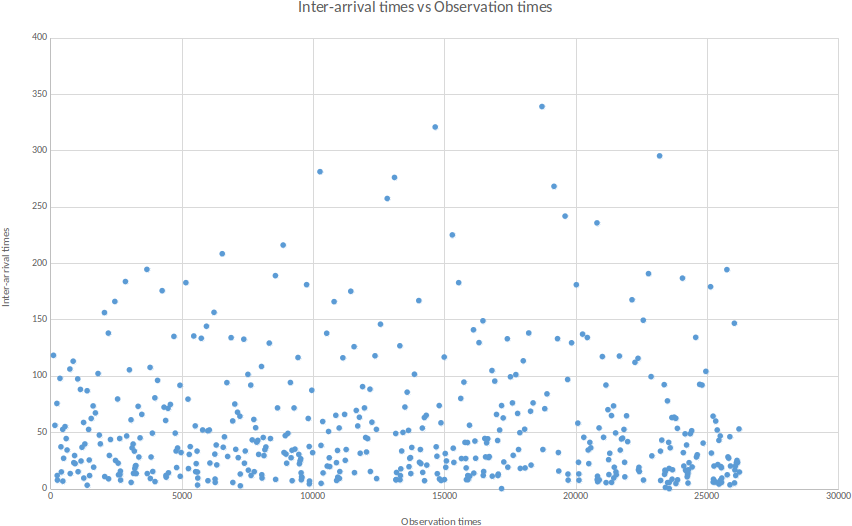
\includegraphics[width=\linewidth]{day2-interarrival-timeseries.png}
        \caption{Interarrival time vs Observer times for day 2}
    \end{subfigure}
\end{figure}

\pagebreak

\section{Autocorrelation test}
In order to do the autocorrelation test we shift data forward once for lag 1 and
twice for lag 2, then calculate using this formula:

\begin{align}
    r_{xy} = \frac{\sum (x_i - \overline{x})(y_i - \overline{y})}{\sqrt{\sum (x_i - \overline{x})^2 \sum(y_i - \overline{y})^2}}
\end{align}

where $x$ is original data, $y$ is the lagged version. Calculations are done
inside the spreadsheet.

After calculating autocorrelation coefficient for lag 1 and lag 2 for both days
we obtain the following plots. We find that there is low autocorrelation $< 0.1$
therefore the underlying random number generator is good.


\begin{figure}[H]
    \begin{subfigure}{0.5\textwidth}
        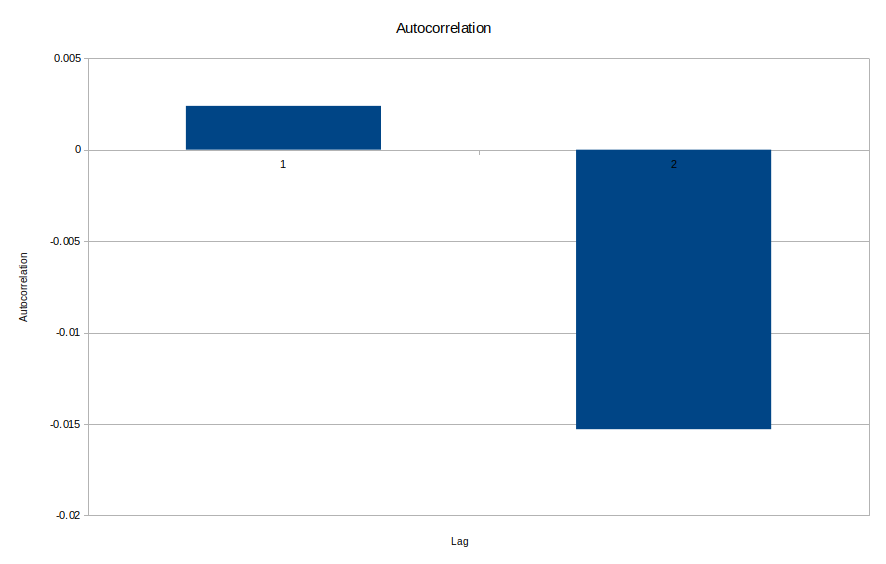
\includegraphics[width=\linewidth]{day1-autocorr.png}
        \caption{Autocorrelation for day 1}
    \end{subfigure}
    \begin{subfigure}{0.5\textwidth}
        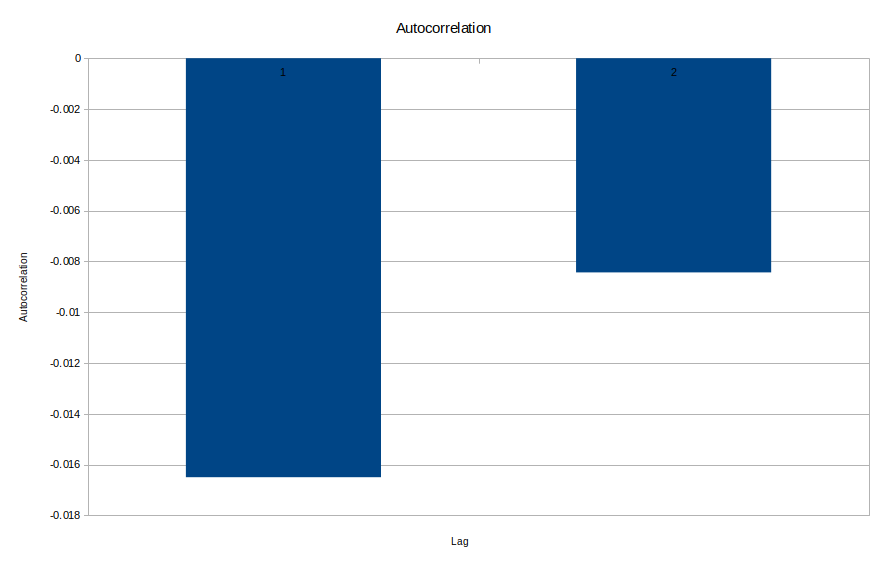
\includegraphics[width=\linewidth]{day2-autocorr.png}
        \caption{Autocorrelation for day 2}
    \end{subfigure}
\end{figure}

% \section{Conclusion}
\end{document}


% \begin{table}[H]
%     \tiny
%     \centering
%     \caption{Statistical analysis of the 10 runs of 1000 answered calls}
%     \begin{tabular}{@{}lllllllllll@{}}
%         \toprule
%         \textbf{} & \textbf{Sys. Util} & \textbf{Op1 Util} & \textbf{Op2 Util} & \textbf{Avg. Wait} & \textbf{W/S} & \textbf{Avg. \# in Op1 Q} & \textbf{Avg. \# in Op2 Q} & \textbf{\# Unsatisfied} \\ \midrule
%         mean      & 0.008              & 0.446             & 0.411             & 2.143              & 0.16         & 0.147                     & 0.173                     & 184.7                   \\
%         std       & 0.0                & 0.024             & 0.014             & 0.142              & 0.009        & 0.01                      & 0.022                     & 11.748                  \\
%         min       & 0.008              & 0.411             & 0.393             & 1.997              & 0.149        & 0.131                     & 0.144                     & 172.0                   \\
%         25\%      & 0.008              & 0.432             & 0.402             & 2.038              & 0.154        & 0.141                     & 0.155                     & 175.25                  \\
%         50\%      & 0.008              & 0.445             & 0.406             & 2.106              & 0.158        & 0.15                      & 0.172                     & 182.0                   \\
%         75\%      & 0.008              & 0.458             & 0.418             & 2.224              & 0.166        & 0.153                     & 0.186                     & 194.25                  \\
%         max       & 0.009              & 0.489             & 0.439             & 2.441              & 0.176        & 0.161                     & 0.209                     & 202.0                   \\ \bottomrule
%     \end{tabular}
% \end{table}
